% Compact single-column motivation, introduced at its first reference.
\begin{figure}[t]
  \centering
  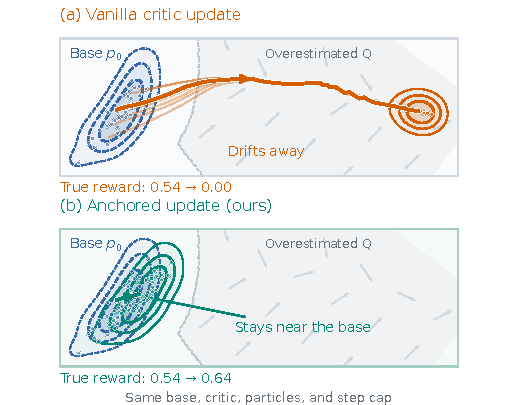
\includegraphics[width=\linewidth]{figures/problem_motivation.pdf}
  \caption{\textbf{Preserving pretrained robot skills during refinement.}
Both panels use the same frozen critic, paired initial actions from the blue base distribution, and per-update step cap in a synthetic action space. (a) Critic ascent moves actions into an overestimated region (gray), reducing true reward. (b) Projection around each initial action maintains a fixed base reference and improves reward. Curves trace representative updates; contours show estimated action distributions.}
  \label{fig:problem}
\end{figure}
